\subsubsection{Select $\sigma$}

\url{https://en.wikipedia.org/wiki/Selection_(relational_algebra)}\\

\begin{figure}[H]
	\centering
	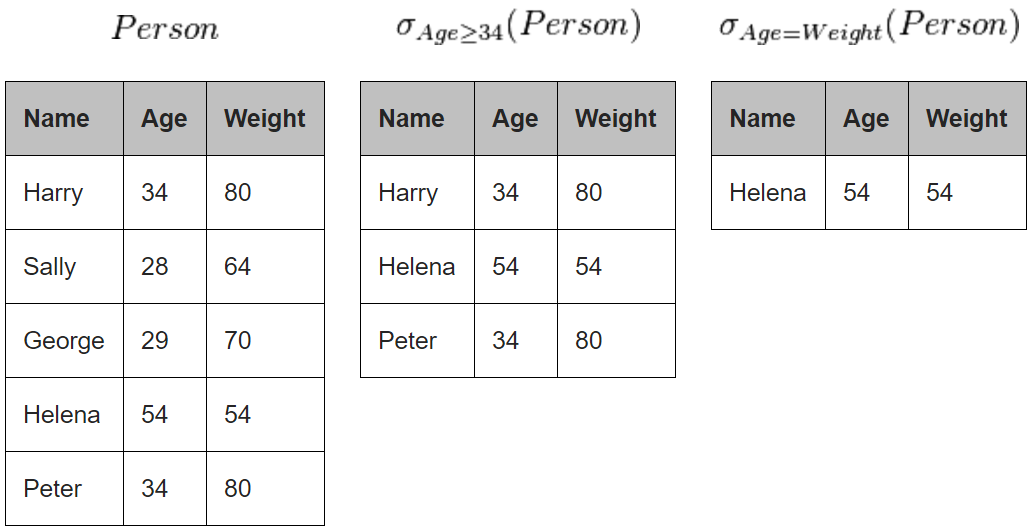
\includegraphics[width=0.9\linewidth]{figs/spm6/select}
	\caption{RA og select.}
	\label{fig:select}
\end{figure}


Laver en \textit{horizontal partition} af en tabel og finde hele rækker som opfylder en eller flere betingelser.

%Nu kan vi så bruge et \textbf{\textit{select}} statement til at finde alle studerende som har alder over 23, og gennemsnit over 8.
%
%Med relationel algebra vil dette se således ud:
%
%\begin{equation*}
%\sigma_{alder \geq 23}\text{ and } _{gennemsnit \geq 8} (\text{Studerende})
%\end{equation*}
%
%Dette vil så returnere følgende tabel:
%
%\begin{table}[H]
%	\centering
%	\begin{tabular}{lrrl}
%		\toprule
%		\textbf{Navn}	&\textbf{Alder}&\textbf{Gennemsnit}&\textbf{Email}\\
%		\midrule			
%		Hans Hansen		& 45 & 9,8	& hans@landmand.dk	\\			
%		Signe Andersen	& 25 & 8,6	& signe@hotmail.com	\\
%		\bottomrule
%	\end{tabular}
%	\caption{Studerende ældre end 23 med snit over 8.}
%\end{table}
%
%
%På denne måde laver \textbf{\textit{select}} operatoren en \textit{horizontal partition} med to dele: én der opfylder betingelserne og én som ikke gør.